\textbf{ID:} UC16 (Manage Media For Display) \\
\textbf{Scope:} CS Automated Information Timeline \\
\textbf{Level:} User goal \\
\textbf{Primary Actor:} Office Manager \\
\textbf{Stakeholders and Interests:}
\begin{itemize}
    \item Admin/Reviewer: Wants to ensure curated list of media items are on display for guests
    \item Guest: Wants to be able to see images and/or video on the TV display
    \item Faculty: Wants to ensure relevant media can be shown to guests.
\end{itemize}
\textbf{Preconditions:}
\begin{itemize}
    \item User with Office Manager role has been authenticated.
    \item Media library is available.
\end{itemize}
\textbf{Postconditions:}
\begin{itemize}
    \item Media is displayed on the TV display
    \item The ordering of the media displayed is correct
\end{itemize}
\textbf{Main Success Scenario:}
\begin{enumerate}
    \item User navigates to media library
    \item The system displays the media library and available files for display
    \item User selects media to be displayed on the main display
    \item The system displays the list of media that will be displayed on the main display
    \item Repeat step 3 and 4 until all required media is selected for display
    \item User reviews final list of media to be displayed
    \item User approves media display and saves new list of media to be displayed
    \item The system records the final list and the user identification associated with the created list
    \item The system updates the main display with the list of media to display
    \item The system provides local copies of media to the main display
    \item The main display begins displaying the listed media
    \item The system notifies the user that the listed media has been saved and is displayed on the main display
\end{enumerate}
\textbf{Alternative Flows:} \\
3A: User does not find suitable media for display and has media to upload
\begin{enumerate}
    \item User selects media they wish to upload from local device
    \item User uploads new media to media library
    \item The system confirms successful upload of media
    \item The system adds newly uploaded media to list of media to display
    \item Proceed to step 4 of the main scenario
\end{enumerate}
3B: User wants to remove items from current Media list
\begin{enumerate}
    \item User proceeds to modify currently returned media list
    \item System returns the current list of media marked for display on the main display
    \item User updates list to remove media
    \item System returns updated list
    \item Repeat step 3 and 4 until either all media is removed from the list or user cancels the action.
    \item Proceed to step 6 of the main scenario
\end{enumerate}
7A: User needs to modify order of media to be displayed
\begin{enumerate}
    \item User selects option to change media ordering
    \item The system notifies the user the current order of media will be lost
    \item User confirms
    \item The system returns user to step 3 of the main scenario
\end{enumerate}

\begin{figure}[H]
    \centering
    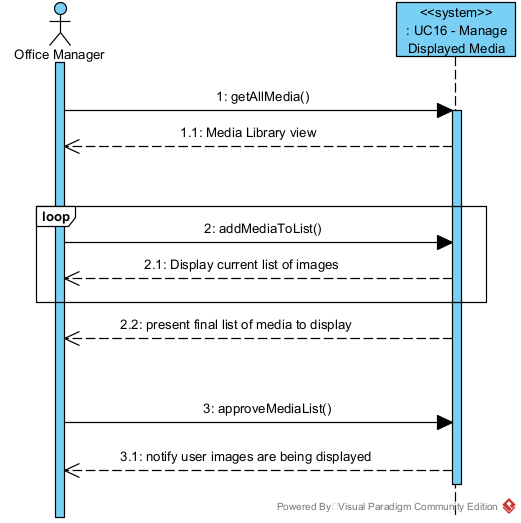
\includegraphics[width=0.8\textwidth]{images/SSD-UC16-ManageDisplayedMedia.png}
    \centering
    \caption{System Sequence Diagram: Manage Displayed Media}
\end{figure}

\textbf{Operation:} getAllMedia() \\
\textbf{Cross-References:} UC16 (Manage Media For Display) \\
\textbf{Pre-conditions:}
\begin{itemize}
    \item Media objects exist in the media library (database store)
    \item Media objects have been approved by admin
\end{itemize}
\textbf{Post-conditions:}
\begin{itemize}
    \item List of media returned to user as List<> object, \emph{ml}
\end{itemize}

\textbf{Operation:} addMediaToList() \\
\textbf{Cross-References:} UC16 (Manage Media For Display) \\
\textbf{Pre-conditions:}
\begin{itemize}
    \item Media List object, \emph{ml}, is not at capacity yet
    \item \emph{ml} has not been approved
\end{itemize}
\textbf{Post-conditions:}
\begin{itemize}
    \item \emph{ml} has association with media item, \emph{m}, formed
    \item \emph{ml} has been updated and requests approval
\end{itemize}

\textbf{Operation:} approveMediaList () \\
\textbf{Cross-References:} UC16 (Manage Media For Display) \\
\textbf{Pre-conditions:}
\begin{itemize}
    \item User has marked \emph{ml} as ready for publish
    \item \emph{ml} is not over capactiy
    \item \emph{ml}  has not been approved yet
\end{itemize}
\textbf{Post-conditions:}
\begin{itemize}
    \item \emph{ml} is approved and set for display
    \item \emph{MainDisplay} updates with new list, \emph{ml}
\end{itemize}
